% chapter3_methodology.tex

\section{Chapter Overview}
This chapter outlines the methodology adopted for the design, development, and evaluation of \textbf{RootLens}. Using Saunders' Research Onion model (Saunders, Lewis and Thornhill, 2019), it establishes the research philosophy and strategy, details the development process and solution pipeline, presents project management decisions, and reviews social, legal, ethical, and professional considerations.

\section{Research Methodology}
The research design for this project follows Saunders' Research Onion (Saunders, Lewis and Thornhill, 2019), a layered framework that structures research decisions from philosophical underpinnings through to data collection techniques. Table~\ref{tab:research_onion} summarises the choice made at each layer and its justification in the context of the RootLens research.

\begin{xltabular}{\textwidth}{|p{2.5cm}|p{3.3cm}|X|}

\hline
\textbf{Layer} & \textbf{Choice} & \textbf{Justification} \\ \hline
\endfirsthead

Philosophy & Positivism & RootLens produces objective, measurable outputs (accuracy, latency, confidence) suited to empirical evaluation without subjective interpretation. \\ \hline

Approach & Deductive & Hypotheses about classification accuracy and confidence weighting are formulated from established theory and tested experimentally. \\ \hline

Choice & Multi-method & Primary evaluation metrics (accuracy, latency, confidence) are quantitative. A supplementary Likert-scale and open-ended expert evaluation captures qualitative insights on usability and operational relevance. \\ \hline

Strategy & Experiment & Controlled fault-injection experiments on Minikube with labelled ground-truth enable isolation of variables and measurement of classification accuracy and latency. \\ \hline

Time Horizon & Cross-sectional & Evaluated across 30 experiments within a defined time window; longitudinal collection is outside scope. \\ \hline

Techniques & Fault injection, ML training, survey, API testing & Fault injection generates labelled data; ML training produces explainer models; a questionnaire gathers requirements; automated API testing validates accuracy. \\ \hline

\caption{Research Onion Layer Choices}
\label{tab:research_onion}
\end{xltabular}

\textbf{Hypothesis:} A hybrid root cause analysis model combining a deterministic rule-based engine with category-specific Random Forest ML classifiers, using a 60/40 weighted confidence combination, can accurately and reliably classify KEDA-triggered Kubernetes autoscaling delays into three root cause categories in real time, achieving $\geq$95\% root cause accuracy, $\geq$80\% sub-cause accuracy, and $<$300ms RCA latency, while maintaining graceful degradation when the ML service is unavailable. This hypothesis addresses all four research questions from Chapter~1: RQ1 (timing signals and thresholds), RQ2 (category-specific feature sets), RQ3 (optimal confidence weighting), and RQ4 (hybrid vs.\ baseline comparison).

\subsection{Critical Evaluation of Research Methodology}
The positivist, deductive, experimental approach is well-suited to evaluating a technical system with quantitative performance metrics. However, it carries inherent limitations. While the multi-method choice incorporates both quantitative metrics and qualitative expert feedback, the qualitative component is limited to ten evaluators and does not constitute a full qualitative study; deeper insights from extended interviews with practising SREs could have provided richer feedback. The cross-sectional time horizon captures system performance at a single point but cannot assess how accuracy degrades as infrastructure configurations drift over time. The 15-response survey (60\% response rate) provides useful requirements input but is too small for statistical generalisation. Despite these limitations, the experimental strategy remains the most valid approach for the core research question, which concerns objective classification accuracy rather than subjective user experience.

\section{Development Methodology}

\subsection{Choice of Development Methodology}
Waterfall was rejected because threshold values and feature definitions depend on experimental results, precluding a single design-then-build pass. Scrum's ceremony overhead is disproportionate for a single-developer project.

\textbf{Selected methodology: Iterative Development.} RCA threshold values ($D_{\text{cold}} > 30\text{s}$, $D_{\text{sched}} > 10\text{s}$, $D_{\text{lag}} > 45\text{s}$) required empirical calibration through prototype testing, and the ML training depended on the data pipeline being implemented first, both necessitating iterative refinement. The project was executed across three iterations: (1) rule-based engine and data collection, (2) ML model training and integration, and (3) dashboard, Kubernetes Operator, and evaluation.

\subsection{Requirement Elicitation Methodology}
Requirements were gathered through three complementary methods: (1)~a systematic literature review of 20+ papers (Chapter~2) identifying functional gaps in prior work; (2)~a structured, closed-ended questionnaire distributed to DevOps and SRE professionals, gathering quantitative data on diagnostic pain points, acceptable latency, and dashboard priorities (results in Chapter~4 and Appendix~A); and (3)~iterative prototyping on Minikube, where prototype behaviour refined threshold values and API response structure before formal requirements were fixed.

\subsection{Design Methodology}
The system was designed using \textbf{OOADM} principles adapted for a component-based microservice architecture. Each concern (data collection, rule-based classification, ML inference, API, dashboard) is encapsulated in a loosely coupled component with well-defined interfaces. The full design is documented in Chapter~6.

\subsection{Programming Paradigm}
The Go backend uses concurrent goroutines, channel-based communication, and interface-based dependency injection. The Python ML service uses pure functions for feature extraction with stateless Flask request handling and scikit-learn pipelines. The React dashboard uses component-based functional style with hooks.

\subsection{Testing Methodology}
Testing follows the \textbf{Test Pyramid}: unit tests in Go (17 tests covering API validation, RCA engine, and collector), Python (26 tests covering ML feature extractors), and the Kubernetes Operator (6 tests using Ginkgo v2 + envtest) verify individual functions in isolation (49 unit tests total); integration tests (19 tests) validate cross-component interactions including Go-to-Python ML pipelines and model loading; system tests (25 checks) validate deployment infrastructure including Helm chart linting, Kustomize builds, and Kubernetes manifest dry-runs; and 30 fault-injection experiments on Minikube verify end-to-end accuracy against ground-truth labels.

\section{Solution Methodology}
The RootLens solution executes a five-phase pipeline for each scaling event: (1)~\textbf{Collect}, where the data collection module watches the Kubernetes API for pod creation events, KEDA ScaledObject state changes, and RabbitMQ queue depth metrics, capturing a timing snapshot; (2)~\textbf{Classify Rule}, where deterministic thresholds on image pull duration, scheduling duration, and metric lag classify the event into Cold Start Latency, Scheduling Contention, or Metric Propagation Lag with a rule-based confidence score; (3)~\textbf{Extract Features}, where a category-specific feature vector (15/11/10 features) is constructed from the timing signals and Kubernetes metadata; (4)~\textbf{ML Predict}, where the vector is sent to the Python Flask ML service, where the appropriate Random Forest returns a sub-cause label, probability, and feature importance explanation; (5)~\textbf{Combine Confidence}, where the final score is computed as $C_{final} = 0.6 \times C_{rule} + 0.4 \times C_{ml}$ and stored in the in-memory ring buffer.

Feature candidates were identified from domain literature (Wang et al., 2018; Rattihalli et al., 2019; Burns et al., 2016; Vayghan et al., 2021) and empirically validated through Random Forest feature importance analysis, retaining only features with discriminative power.

\subsection{Justification of Random Forest}
\label{subsec:rf_justification}

Four supervised classifiers were evaluated against the RootLens constraints before Random Forest was selected. Table~\ref{tab:model_comparison} summarises the analysis.

\begin{xltabular}{\textwidth}{|p{2.8cm}|X|X|}

\hline
\textbf{Model} & \textbf{Limitations in this context} & \textbf{Assessment} \\ \hline
\endfirsthead

\hline
\textbf{Model} & \textbf{Limitations in this context} & \textbf{Assessment} \\ \hline
\endhead

Support Vector Machine & Requires careful kernel selection and $C$/$\gamma$ hyperparameter tuning; no native feature importances, so probability calibration via Platt scaling adds complexity; does not satisfy the explainability requirement. & Rejected: poor interpretability. \\ \hline
Neural Network & Requires hundreds to thousands of samples to generalise; with only 34-42 labelled samples per category, even shallow networks are prone to severe overfitting; opaque weights conflict with the explainability requirement. & Rejected: insufficient data and black-box nature. \\ \hline
Gradient Boosted Trees (XGBoost) & Competitive accuracy but sensitive to learning rate, max depth, $n\_estimators$, and regularisation hyperparameters; marginal accuracy gains over Random Forest do not justify the added tuning burden for datasets of this size. & Rejected: complexity overhead unwarranted. \\ \hline
\textbf{Random Forest} & Bagging over decision trees provides natural variance reduction on small datasets (Breiman, 2001); native \texttt{feature\_importances\_} satisfy the explainability requirement without post-hoc approximation; minimal hyperparameter sensitivity; validated on structured Kubernetes telemetry data by Toka et al.\ (Toka, Varga and Marosi, 2021). & \textbf{Selected.} \\ \hline

\caption{Supervised Classifier Comparison for RootLens}
\label{tab:model_comparison}
\end{xltabular}

Random Forest satisfies all three requirements: small-dataset generalisation through bagging (Breiman, 2001), native feature importances, and validated performance on Kubernetes data (Toka, Varga and Marosi, 2021).

\section{Project Management Methodology}

\subsection{Schedule}
The project was planned across three academic terms using a Gantt chart (Figure~\ref{fig:gantt}), divided into three overlapping phases: research and planning, design and build, and evaluation and write-up.

\begin{figure}[H]
\centering
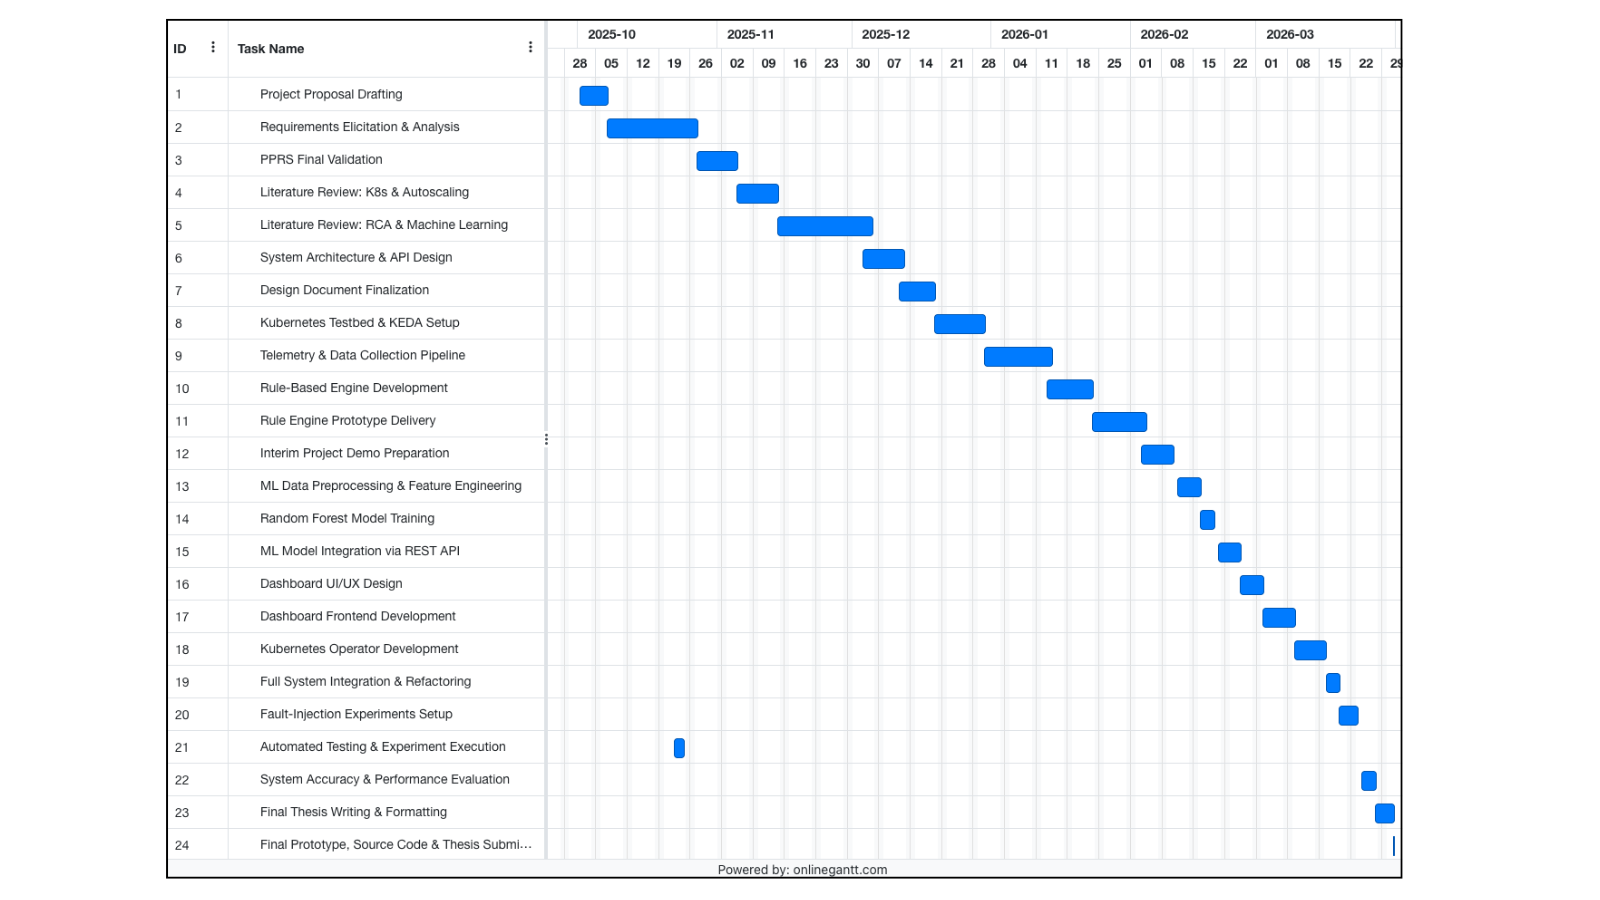
\includegraphics[width=1.0\textwidth]{thesis/assets/gantt_chart.png}
\caption{Project Gantt Chart}
\label{fig:gantt}
\end{figure}

\subsection{Deliverables}
Table~\ref{tab:deliverables_expanded} lists the project deliverables and their planned submission dates.

\begin{xltabular}{\textwidth}{|X|p{3.5cm}|}

\hline
\textbf{Deliverable} & \textbf{Date} \\ \hline
\endfirsthead

\hline
\textbf{Deliverable} & \textbf{Date} \\ \hline
\endhead

Topic Selection \& Initial Research & 5th Oct 2025 \\ \hline
Project Proposal Drafting & 10th Oct 2025 \\ \hline
Requirements Elicitation \& Analysis & 25th Oct 2025 \\ \hline
PPRS Final Validation & 6th Nov 2025 \\ \hline
Literature Review: K8s \& Autoscaling & 13th Nov 2025 \\ \hline
Literature Review: RCA \& Machine Learning & 21st Nov 2025 \\ \hline
System Architecture \& API Design & 25th Nov 2025 \\ \hline
Design Document Finalization & 28th Nov 2025 \\ \hline
Kubernetes Testbed \& KEDA Setup & 4th Dec 2025 \\ \hline
Telemetry \& Data Collection Pipeline & 12th Dec 2025 \\ \hline
Rule-Based Engine Development & 24th Dec 2025 \\ \hline
Rule Engine Prototype Delivery & 31st Dec 2025 \\ \hline
Interim Project Demo Preparation & 9th Jan 2026 \\ \hline
ML Data Preprocessing \& Feature Engineering & 15th Jan 2026 \\ \hline
Random Forest Model Training & 20th Jan 2026 \\ \hline
ML Model Integration via REST API & 26th Jan 2026 \\ \hline
Dashboard UI/UX Design & 2nd Feb 2026 \\ \hline
Dashboard Frontend Development & 9th Feb 2026 \\ \hline
Kubernetes Operator Development & 20th Feb 2026 \\ \hline
Full System Integration \& Refactoring & 2nd Mar 2026 \\ \hline
Fault-Injection Experiments Setup & 10th Mar 2026 \\ \hline
Automated Testing \& Experiment Execution & 20th Mar 2026 \\ \hline
System Accuracy \& Performance Evaluation & 27th Mar 2026 \\ \hline
Final Thesis Writing \& Formatting & 30th Mar 2026 \\ \hline
Final Prototype, Source Code \& Thesis Submission & 31st Mar 2026 \\ \hline

\caption{Detailed Project Deliverables and Milestones}
\label{tab:deliverables_expanded}
\end{xltabular}

\subsection{Resource Requirements}
Data was generated from 30 controlled fault-injection runs on Minikube; no external datasets were used. Hardware and software requirements are detailed in Chapter~1 (Tables~\ref{tab:hardware_req} and \ref{tab:software_req}).

\subsection{Risk and Mitigation}
Table~\ref{tab:risks} identifies the primary project risks. Risk Exposure is calculated as $\text{Probability} \times \text{Severity}$ on a 1-5 scale for each.

\begin{xltabular}{\textwidth}{|p{3.5cm}|p{1.8cm}|p{1.8cm}|p{1.5cm}|X|}

\hline
\textbf{Risk} & \textbf{Severity (1-5)} & \textbf{Probability (1-5)} & \textbf{Exposure} & \textbf{Mitigation Strategy} \\ \hline
\endfirsthead

\multicolumn{5}{c}{\textit{Table \thetable\ continued from previous page}} \\
\hline
\textbf{Risk} & \textbf{Severity (1-5)} & \textbf{Probability (1-5)} & \textbf{Exposure} & \textbf{Mitigation Strategy} \\ \hline
\endhead

\hline
\endfoot

\hline
\endlastfoot

Feature-scaler mismatch between training and inference & 5 & 3 & 15 & Defined and documented feature contracts; automated feature count assertion at model load time. \\ \hline
Insufficient labelled training data for ML models & 5 & 4 & 20 & Controlled fault injection on Minikube with verified ground-truth labels; synthetic data augmentation as fallback if needed. \\ \hline
ML service unavailability in production & 3 & 3 & 9 & Implemented graceful degradation to rule-based analysis; ML failure does not propagate to API error. \\ \hline
Minikube instability during experiments & 4 & 2 & 8 & Snapshot Minikube state before experiments; scripted reproducible experiment setup with automated cluster reset. \\ \hline
Scope creep beyond project timeline & 4 & 3 & 12 & Fixed scope documented in SRS; change requests evaluated against timeline impact before acceptance. \\ \hline
Overfitting of ML models on small dataset & 4 & 4 & 16 & Monitored train/test accuracy gap; used Random Forest which is inherently resistant to overfitting through bootstrap aggregation (bagging); dataset size acknowledged as a limitation. \\ \hline
Hardcoded credentials in source code & 5 & 2 & 10 & Conducted security audit; replaced all hardcoded values with environment variable and Kubernetes Secret references. \\ \hline

\caption{Project Risk Register}
\label{tab:risks}
\end{xltabular}

The social, legal, ethical, and professional considerations relevant to this project are discussed in detail in Chapter~5.

\section{Methodological Contribution}
Beyond serving the immediate needs of this project, the methodology contributes a reusable experimental framework for evaluating RCA systems in Kubernetes environments. The combination of chaos engineering fault injection (Basiri et al., 2016) for labelled dataset generation, category-specific ML training with real experimental data, and hybrid rule-ML confidence combination provides a template that future researchers can adapt for different event sources, cluster configurations, or failure taxonomies. This methodological pattern addresses the data scarcity problem identified in the literature (Notaro, Cardoso and Gerndt, 2021) as a primary barrier to applying ML in operational environments.

\section{Chapter Summary}
This chapter established a positivist, deductive, experimental methodology using Saunders' Research Onion framework, with iterative development chosen over Waterfall and Scrum for its suitability to a single-developer research project requiring empirical threshold calibration. The five-phase solution pipeline (Collect, Classify Rule, Extract Features, ML Predict, Combine Confidence) was defined, Random Forest was justified against three alternative classifiers, and requirements elicitation combined literature review, questionnaire survey, and iterative prototyping. Project management was structured through a Gantt chart with three overlapping phases, and seven key risks were identified with mitigation strategies. Chapter~4 specifies the system requirements derived from this foundation.